\chapter{Implementation and experimental results}
\label{ch:implementation}

To build up the confidence of the horizontal scalability claim from our analytical results,
we must verify the same property experimentally.
Hence, we give an open source prototype implementation of our system.
Our implementation runs on a network with over 1000 node.
Each node sends transactions to each other autonomously, 
which allows us to evaluate our analytical claims.

We begin this chapter with a description of the implementation in \Cref{sec:implementation}.
Then, we move on to describing our experimental setup in \Cref{sec:experimental-setup} which includes a discussion on the system parameters and the physical infrastructure which we use.
Finally, \Cref{sec:comms-cost-experiment} and onwards follows the same structure as the Performance analysis (\Cref{sec:performance-analysis}),
where we analyse the performance experimentally rather than analytically and compare both results.


\section{Implementation}
\label{sec:implementation}

The prototype implementation can be found on GitHub.
\begin{displayquote}
\url{https://github.com/kc1212/consensus-thesis-code}
\end{displayquote}
It implements the three protocols and the Extended TrustChain discussed in~\Cref{ch:model}.
We also implement two optimisations---privacy preserving validation protocol using compact blocks (\Cref{sec:compact})
and optimised validation protocol using cached agreed fragments (\Cref{sec:caching}).
It is written in the event driven paradigm, using the Python programming language\footnote{\url{https://www.python.org/}}.
We use the Twisted\footnote{\url{https://twistedmatrix.com/}} library for networking.

The structure of the implementation is primarily made up of three modules---\texttt{acs}, \texttt{trustchain} and \texttt{node}.
\texttt{acs}, as its name suggests, implements ACS.
ACS uses erasure code in one of its sub-protocols (reliable broadcast).
Thus we use the liberasurecode\footnote{\url{https://github.com/openstack/liberasurecode}} library for its Reed-Solomon error correcting code functionality.
An implementation detail is that liberasurecode cannot create more than 32 code blocks\footnote{
  The 32 code blocks limitation is hardcoded in the source file, see
  \url{https://github.com/openstack/liberasurecode/blob/0794b31c623e4cede76d66be730719d24debcca9/include/erasurecode/erasurecode.h\#L35}
}, we discuss the effect of this in~\Cref{sec:experimental-setup}.
The \texttt{acs} module provides a small interface to the caller to start and stop the consensus process and also retrieve results.
The \texttt{trustchain} module implements the Extended TrustChain data structure.
It also provides the essential algorithm necessary to interact with Extended TrustChain such as 
$\textsf{new\_tx}(\cdot)$, $\textsf{new\_cp}(\cdot)$ and $\textsf{agreed\_fragment}(\cdot)$.
Finally, the \texttt{node} module ties everything together.
It implements the consensus protocol, the transaction protocol and the validation protocol.


Every node keeps a persistent TCP connection with every other node.
This creates a fully connected network for our experiment.
It is certainly not ideal in real world scenarios where nodes may have limited resources (e.g. sockets).
But as a prototype, it is sufficient to run a network of over a thousand nodes and experiment with it.

Finally, the cryptography primitives we use are SHA256 for hash functions and Ed25519 for digital signatures.
Both of which are provided by libnacl~\footnote{\url{https://pypi.python.org/pypi/libnacl}}.


\section{Experimental setup}
\label{sec:experimental-setup}

The goal of the experiment is to run the three protocols---consensus protocol,
transaction protocol and validation protocol---simultaneously and analyse the communication cost, the consensus duration and the global throughput.
We investigate these properties under the following four parameters.
\begin{enumerate}
  \item The transaction rate $r_{\text{tx}}$ per node. This is not comparable to the others because it is fixed at 2 TX/s.
        Nevertheless, it is a good value because, as we show later,
        it hits a bottleneck in extreme cases which helps us understand the limitations of our design.
  \item The number of facilitators $n \in \{4, 8, \dots, 32\}$.
        The maximum $n$ is 32 because the limitation in liberasurecode mentioned in \Cref{sec:implementation},
        but our results give a good indication of how our system may function for larger numbers of $n$.
  \item The population size $N \in \{200, 300, \dots, 1200\}$.
        $N$ stops at 1200 is due to our physical setup, which we describe next.
  \item The two modes of transaction.
        The first mode is the \emph{fixed-neighbour} mode where nodes only transact with their immediate neighbour which is predetermined. 
        This minimises the data volume per validated transaction because agreed fragment can be cached.
        The second mode is in the other extreme which we call the \emph{random-neighbour} mode,
        where every transaction is with a random node out of the $N$ nodes in the system.
        It is unlikely that the agreed fragments can be reused.
\end{enumerate}

The experiment is run on the DAS-5\footnote{\url{https://www.cs.vu.nl/das5/}}.
From now on, we use ``machines'' to refer to DAS-5 nodes and ``nodes'' to refer to a running instance in our system.
On DAS-5 we use up to 30 machines, for each machine we use up to 40 nodes.
This gives us the aforementioned 1200 number.
With this setup, we cannot run more nodes because the every machine only has 65535 ports available (minus the reserved ones).
But 40 nodes each need 1200 TCP connections which is 48000 TCP connections per machine and that is inching close to the limit.
While it is possible to have more TCP connections per machine,
but it requires additional network interface which is something we do not control on the DAS-5.
Nevertheless, running the system with 1200 nodes gives a good indication of its scalability properties as we show later.

To coordinate nodes on many different machines,
we employ a discovery server to inform every node the IP addresses and port numbers of every other node.
It is only run before the experiment and is not used during the experiment.

Finally, since Bitcoin transactions are approximately 500 bytes~\cite{txsize},
we use a uniformly random transaction size sampled between 400 and 600 bytes.


\section{Communication cost for the consensus protocol}
\label{sec:comms-cost-experiment}

The remainder of this chapter follows the same structure as the performance analysis in~\Cref{sec:performance-analysis}.
We check our analytical results experimentally and demonstrate horizontal scalability.

\begin{figure}[tb]
  \centering
  \makebox[\linewidth][c]{%
    \begin{subfigure}[b]{.7\textwidth}
      \includegraphics[width=\textwidth]{neighbour-fixed/round-communication-cost-vs-population}
      \caption{Transactions are with fixed neighbours.}
      \label{fig:round-comms-fixed}
    \end{subfigure}%
    \begin{subfigure}[b]{0.7\textwidth}
      \includegraphics[width=\textwidth]{neighbour-random/round-communication-cost-vs-population}
      \caption{Transactions are with random neighbours.}
      \label{fig:round-comms-random}
    \end{subfigure}%
  }
  \caption{Communication cost for the consensus protocol per round increases linearly with population size.
  The error bars are larger for higher population size or higher number of facilitators is because rounds take longer thus they are repeated fewer times.}
  \label{fig:round-comms}
\end{figure}

\begin{figure}[tb]
  \centering
  \makebox[\linewidth][c]{%
    \begin{subfigure}[b]{.7\textwidth}
      \includegraphics[width=\textwidth]{neighbour-fixed/round-duration-vs-population}
      \caption{Transactions are with fixed neighbours.}
      \label{fig:round-duration-fixed}
    \end{subfigure}%
    \begin{subfigure}[b]{0.7\textwidth}
      \includegraphics[width=\textwidth]{neighbour-random/round-duration-vs-population}
      \caption{Transactions are with random neighbours.}
      \label{fig:round-duration-random}
    \end{subfigure}%
  }
  \caption{Round duration does not increase linearly with the population size. 
  This is likely due to the additional hashing operation required for larger consensus result.}
  \label{fig:round-duration}
\end{figure}

\Cref{fig:round-comms} shows the relationship between the communication cost of the consensus protocol per round and the population size.
The most important aspect is that these results show a linear increase.
This reinforces our analytical result in~\Cref{sec:cons-complexity}.
Note that regardless of whether the transactions are performed with a random neighbour or with a fixed neighbour,
the magnitude of the communication cost is similar.
Both peak at about 100 MB.
This is expected because the consensus protocol is decoupled from the transaction protocol and the validation protocol.
Finally, the rate for which the communication cost increases is higher when the number of facilitators is higher.
This is also expected because the ACS algorithm has an $n^2$ term in its communication complexity.

We are also interested in how communication costs translate to time.
Hence, for the same experiment, we record the duration in seconds and the result is shown in~\Cref{fig:round-duration}.
Interestingly, the duration is not entirely linear.
We attribute this behaviour to the extra time needed to hash the CP blocks in the consensus result to compute the luck value.
Since if $N$ increases, every node must also perform more hash operations.
These results do not conform to analytical result in~\Cref{sec:cons-duration}.
Nevertheless, the difference is minor and there are ways to optimise the luck value computation.
For example, the luck value can be computed by the facilitators and are sent with the consensus result.
Then the non-facilitator nodes simply use it if there are enough signatures.

\section{Communication cost for transaction and validation protocols}

\begin{figure}[h]
  \centering
  \makebox[\linewidth][c]{%
  \begin{subfigure}[b]{0.7\textwidth}
    \includegraphics[width=\textwidth]{neighbour-fixed/tx-communication-cost-vs-population}
    \caption{Transactions are with fixed neighbours.}
    \label{fig:tx-comms-fixed}
  \end{subfigure}%
  \begin{subfigure}[b]{0.7\textwidth}
    \includegraphics[width=\textwidth]{neighbour-random/tx-communication-cost-vs-population}
    \caption{Transactions are with random neighbours.}
    \label{fig:tx-comms-random}
  \end{subfigure}
  }
  \caption{Communication cost per verified transaction has similar (near linear) trend as~\Cref{fig:round-duration}.
  Fluctuation for the fixed-neighbour mode exists because the cache mechanism is unpredictable.}
  \label{fig:tx-comms}
\end{figure}

We argued that the communication cost per verified transaction is of $O(N)$ (\Cref{sec:communication-cost-for-tx}).
To verify the argument, we plot the relationship between the communication cost of for every validated transaction and population size in~\Cref{fig:tx-comms}.
We observe a near linear relationship, which is due to the near linear relationship of the communication duration mentioned before.
Again, we believe the difference is minor and it is possible to remove the extra overhead.

More interestingly, there is a large difference in communication cost between the two modes of transaction.
When transacting with only one neighbour, the communication cost is low because only one agreed fragment needs to be communicated for every round in order to validate all transactions of that round.
This is because agreed fragments are cached.
On the other hand,
if every node is transacting with a random node, then it is likely the case that one agreed fragment needs to be communicated for every transaction.
Hence the communication cost we see in~\Cref{fig:tx-comms-random} is much higher than in~\Cref{fig:tx-comms-fixed}.

Some fluctuations exist in~\Cref{fig:tx-comms-fixed}, this is due to our caching mechanism.
We send validation requests at the same rate as transactions.
Upon receiving a (remote) agreed fragment, the caching mechanism inspects all the transactions in the agreed fragment and attempts to verify as many as it can,
rather than just the transaction in the original validation request.
However, it may be the case that the agreed fragments arrive later than the validation request interval.
Then it is possible to have sent two or more validation requests for some transactions in the same local agreed fragment.
In this case, the remote would respond with two or more of the same agreed fragments,
which results in extra (wasted) communication cost, and this is the source of the fluctuation seen in~\Cref{fig:tx-comms-fixed}.
The result in~\Cref{fig:tx-comms-random} reinforces our argument.
It is a lot more stable because for every transaction it is almost always the case that an agreed fragment is needed to validate it.

\section{Linear global throughput}
\begin{figure}[h]
  \centering
  \makebox[\linewidth][c]{%
  \begin{subfigure}[b]{0.7\textwidth}
    \includegraphics[width=\textwidth]{neighbour-fixed/throughput-vs-population}
    \caption{Transactions are with fixed neighbours.}
    \label{fig:global-throughput-fixed}
  \end{subfigure}%
  \begin{subfigure}[b]{0.7\textwidth}
    \includegraphics[width=\textwidth]{neighbour-random/throughput-vs-population}
    \caption{Transactions are with random neighbours.}
    \label{fig:global-throughput-random}
  \end{subfigure}
  }
  \caption{Global throughput increases as the population increases when every node transact at the same rate.
  Using fixed neighbours results in a higher throughput because of the caching mechanism.}
  \label{fig:global-throughput}
\end{figure}


Finally, the global throughput results are shown in~\Cref{fig:global-throughput}.
Evidently, the throughput has a linear relationship with the population size.
This result is a strong indication of the horizontal scalability which we aimed to achieve.
It also matches with our analytical result.

Note that the throughput decreases slightly as the number of facilitators increases.
This is due to the additional communication cost for running ACS with a high number of facilitators.
That is, if the network is congested then the nodes may not have enough bandwidth to send validation responses timely.

For~\Cref{fig:global-throughput-fixed},
the magnitude of our throughput may not be self-evident at first glance.
Recall that we fixed our $r_\text{tx}$ to 2, but how is it possible to have around 4800 transactions per second for 1200 nodes (which is 4 TX/s)?
This is due to the way validated transactions are calculated.
Transactions are between two parties, hence if every node makes two transactions per second,
every node also expects to receive two transactions per second.
Hence, for every node, the TX blocks are created at 4 per second.
Validation requests are sent at the same rate, which explains the magnitude.

The difference in magnitude between \Cref{fig:global-throughput-fixed} and \Cref{fig:global-throughput-random} is caused by the caching mechanism mentioned earlier.
If a new agreed fragment needs to be transmitted to validate every transaction then it puts a toll on the network infrastructure.
The low transaction rate in~\Cref{fig:global-throughput-random} is caused by the fact that the network infrastructure cannot keep up with our demand.

We demonstrate the bottleneck issue from a different perspective in~\Cref{fig:backlog}.
The graph is plotted by counting the number of transactions and the number of validated transactions every 5 seconds for one node running in a network of 1200 nodes and 32 facilitators.
In~\Cref{fig:backlog-fixed}, the number of validated transaction changes as a step function.
This means that transactions are validated in bursts, and the validation protocol can ``keep up'' with the transactions.
Note that the horizontal ``lines'' where no new validated transactions are made are on average 76 seconds, this matches with the round duration result in~\Cref{fig:round-duration-fixed}.
On the other hand in~\Cref{fig:backlog-random}, the validation protocol clearly cannot ``keep up'' with the rate which the transactions are made.
As a result, the global throughput is lower when transacting with random nodes than only with neighbours.

\begin{figure}[tb]
  \centering
  \makebox[\linewidth][c]{%
  \begin{subfigure}[b]{0.7\textwidth}
    \includegraphics[width=\textwidth]{neighbour-fixed/timeseries}
    \caption{Transactions are with fixed neighbours.}
    \label{fig:backlog-fixed}
  \end{subfigure}%
  \begin{subfigure}[b]{0.7\textwidth}
    \includegraphics[width=\textwidth]{neighbour-random/timeseries}
    \caption{Transactions are with random neighbours.}
    \label{fig:backlog-random}
  \end{subfigure}
  }
  \caption{A limitation of our system is when nodes are transacting with many random nodes,
  then the network cannot keep up with the large number of agreed fragments that need to be communicated between nodes.
  Hence the slope of validated transactions grows at a slower rate in~\Cref{fig:backlog-random}.}
  \label{fig:backlog}
\end{figure}

\section{Communication cost with varying number of facilitators}
Up to this point we focused on the effect of communication cost, throughput and so on with respect to the population size.
In this section, we consider a varying number of facilitators,
which gives us an insight into our system performance may perform when the number of facilitators is higher than 32.

\begin{figure}[tb]
  \centering
  \makebox[\linewidth][c]{%
  \begin{subfigure}[b]{0.7\textwidth}
    \includegraphics[width=\textwidth]{neighbour-fixed/consensus-communication-cost-vs-facilitators}
    \caption{Transactions are with fixed neighbours.}
    \label{fig:facilitators-comms-fixed}
  \end{subfigure}%
  \begin{subfigure}[b]{0.7\textwidth}
    \includegraphics[width=\textwidth]{neighbour-random/consensus-communication-cost-vs-facilitators}
    \caption{Transactions are with random neighbours.}
    \label{fig:facilitators-comms-random}
  \end{subfigure}
  }
  \caption{The communication cost of the consensus protocol increases polynomially with respect to the number of facilitators as expected from the ACS communication complexity.}
  \label{fig:facilitators-comms}
\end{figure}

\Cref{fig:facilitators-comms} shows the communication cost of the consensus protocol for varying numbers of facilitators.
There is strong evidence that the communication cost grows polynomially.
We expect this because of there are polynomial terms in the ACS communication complexity---$O(n^2|v| + \lambda n^3 \log n)$.
This also means that the rounds would take longer to complete and transactions would take longer to verify.
On the other hand, we get better fault tolerance.
Thus a linear increase in fault tolerance ($t$) costs a polynomial increase in communication cost.
